\begin{figure}[t]
    \centering
    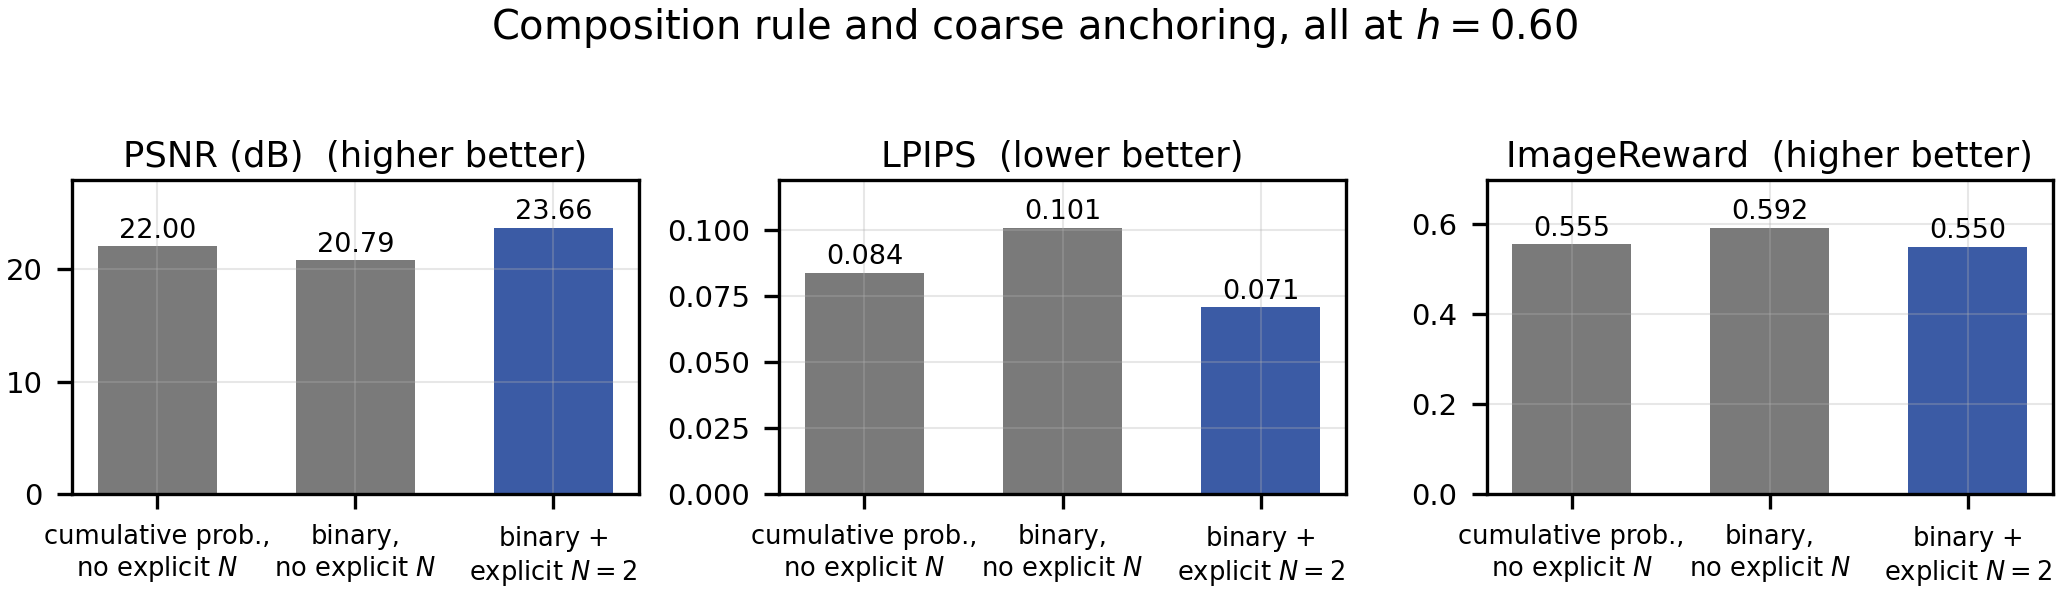
\includegraphics[width=\linewidth]{imgs/fig_anchoring.png}
    \caption{Composition rule and coarse anchoring at $h{=}0.60$. Converting the per-scale binary masks into a cumulative probability field is an implicit and biased form of anchoring; removing it without replacement is worse still, because the coarse scales then carry no anchor. Strictly binary composition with an explicit $N{=}2$ dominates both on preservation at equal edit strength.}
    \label{fig:anchoring}
\end{figure}
